
\subsection{Clustering}
\label{sec:clustering}

The first step towards obtaining a decision tree is to label the data according to their attributes. The inherent attribute of our data are the GOF values, but because of the multiplicity of metrics and lack of clarity about their relationships, we need to label the data according to the validation categories. We do this by means of a clustering process.

Clustering is an unsupervised data-mining process used to group data in a multi-dimensional space based on their attributes \citep{Fayyad_1996_IEEE}. According to \citet{Jain_1999_ACMCS}, clustering can be classified in two categories: hierarchical and partitional. Technical details aside, the basic difference is that hierarchical algorithms create nested partitions, whereas partitional algorithms produce singular partitions.

There is no single clustering process that can be applied to every dataset \citep{Dy_2004_MLR, Jain_1988_Book, Hartigan_1985_JOC}. Consequently, one needs to make a choice. We use a partitional, distance-based method known as constrained \kmeans{}. The standard \kmeans{} method is \change{an unsupervised} process for partitioning a $n$-dimensional population into $k$ clusters with a minimum within-cluster attributes variance \citep[e.g.,][]{Macqueen_1967_Proc}. \change{The constrained \kmeans{} method, on the other hand, is a semi-supervised approach that extends the standard} method by allowing the use of background information in the form of clustering restrictions\change{---thus the upgrade to a semi-supervised method}.

Given a $k$ number of clusters, where each cluster is identified by its center, the standard process starts by computing the distances of all other data-points to the center of the clusters, and grouping them based on their proximity to the clusters' centers. Once this is done, the center of each cluster is updated based on the average attributes of its data-points, and the process is repeated until the clusters become stable.

This process is sensitive to the initial selection of the number of clusters and their centers. To mitigate this, constrained \kmeans{} introduces two types of constraints: must-link and cannot-link \citep{Wagstaff_2001_Proc}. The must-link constraint specifies instances in which two data-points must be linked, i.e., be in the same cluster. The cannot-link constraint specifies instances in which data cannot be in the same cluster. This prevents the process from converging into a local minimum, and defines constrained \kmeans{} as a semi-supervised method. Figure \ref{fig:k-means} illustrates the differences between the standard and constrained \kmeans{} methods for a single clustering iteration on a small two-dimensional dataset.

\begin{figure*}[t]
	\centering
	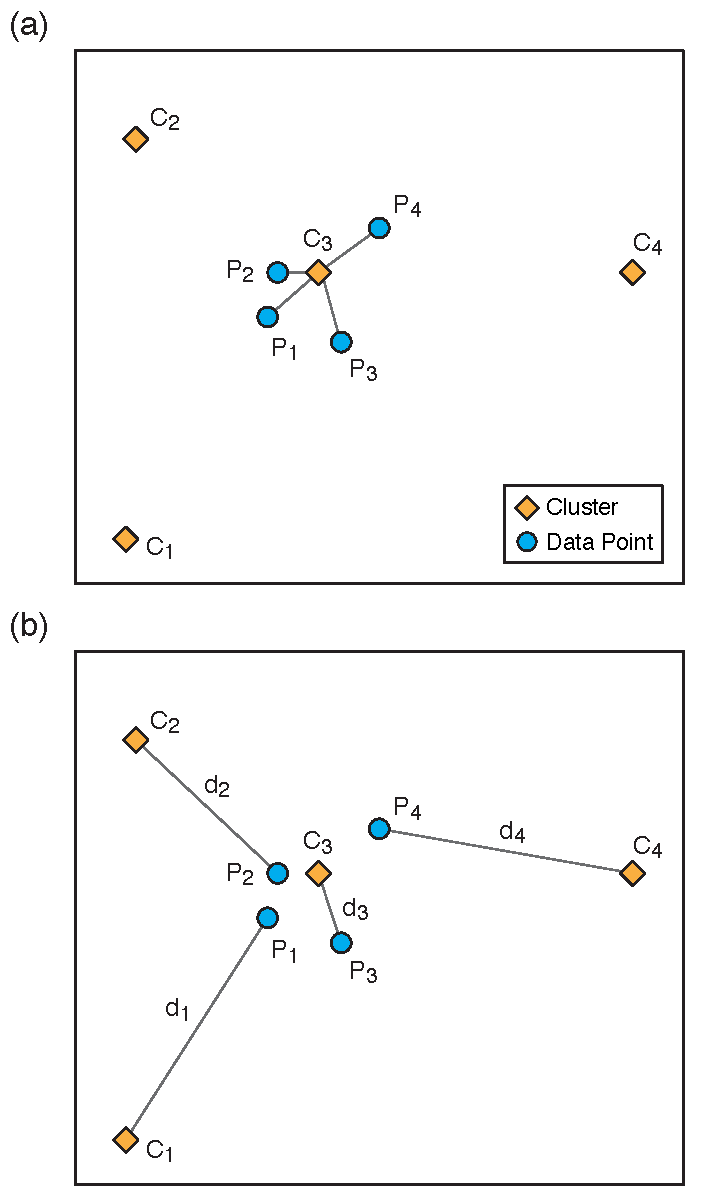
\includegraphics[width=\textwidth]{figures/pdf/figure-04}
	\caption{Representation of the (a) ordinary, and (b) constrained \kmeans{} approaches for four data-points (P) and four cluster centers (C) in a two-dimensional space, where, for the case of the constrained \kmeans{} approach, all the data-points are set to be cannot-link points. The color version of this figure is available only in the electronic edition.}
	\label{fig:k-means}
\end{figure*}

In our implementation we limit the clustering to four validation categories: poor (P), fair (F), good (G), and excellent (E). The cluster centers are randomly selected at the start, but we apply constraints by adding \change{a subset of four artificial data samples into our dataset such that they have cannot-link conditions. These artificial data samples are associated with the different validation categories and are such that they have GOF scores equal to 3, 5, 7, and 9, across all metrics.}
% This means that, in total, we introduce 44 artificial data samples (4 categories $\times$ 11 metrics). These artificial data samples play the role of representatives of the validation categories for each metric.}

\change{The concepts of cluster centers and distances, as exemplified in Fig.~\ref{fig:k-means}, imply the existence of a two-dimensional space. Here, the dimensions are defined by the GOF metrics. We are therefore dealing with an eleven-dimensional space. In clustering, the term dimensions is equivalent to the concept of the data \textit{features}. Within this context, the GOF metrics are the features defining a multi-dimensional space. In such multi-dimensional space defined by the 11 features,} the distances are obtained using the Euclidean expression
%
\begin{equation}
	d(x_i, x_j) = \sqrt{ \sum_{l=1}^{n} \left( x_{i,l} - x_{j,l} \right)^2 }
\end{equation}
%
corresponding to the distance $d$ between the data-point $x_i$ and the cluster center $x_j$ in the $n$-dimensional domain, where $x_{i,l}$ is the $l$-th feature of the data-point $x_i$, and $x_{j,l}$ is the $l$-th feature of the cluster center $x_j$. It is, however, unpractical to expect the patterns defining the clusters to be observable across all features. Such high-dimensional issues are well known \citep[see, for instance,][]{Parsons_2004_ACM, Dy_2004_MLR}, and can be tackled using subspaces. Therefore, instead of analyzing all $2^{11}$ possible subspaces, we focus only on subspaces with 2, 3, and 4 features. In total, we analyze 550 subspaces, 55 subspaces with 2 features, 165 with 3 features, and 330 with 4 features.

Unfortunately, not all the subspaces will have clearly distinguishable clusters (i.e., some will not satisfy the cannot-link constraints even after a large number of iterations). Such subspaces are discarded, and all others are used to label the data. In an ideal case, each \change{subset of data samples corresponding to the comparisons---between synthetic and recorded signals at a particular location (or station) in a simulation---done using the 11 metrics} will be labeled 550 times, and the final label is taken as the mode. For example, if after all the subspaces are accounted for, a station has labels $\left\{F, F, F, P, F, G, E, F, F\right\}$, then such as station will be given a final label $F$. Once \change{all the samples in the dataset have been} properly labeled, we proceed with the decision tree analysis.
